\chapter{Distancia propia, geometría de Kruskal y observadores del horizonte}

La métrica de Schwarzschild parece volverse singular en el horizonte. La curvatura no. Para distinguir ambas afirmaciones, primero eliminamos la escala global del agujero negro y luego sustituimos la coordenada radial por la distancia propia al horizonte. Cerca del horizonte, la geometría resultante es la del espacio-tiempo plano ordinario expresado en coordenadas aceleradas. Una vez dibujada esa geometría, las preguntas sobre Alice, Bob y Charlie pasan a ser preguntas sobre líneas de universo y rayos de luz, en vez de paradojas verbales.

\section{Eliminar la escala del radio de Schwarzschild}

Empecemos con coordenadas primadas, de modo que las variables reescaladas puedan llevar después los nombres habituales:
\begin{equation}
d\tau^2
=
\left(1-\frac{2MG}{r'}\right)dt'^2
-
\frac{dr'^2}{1-\frac{2MG}{r'}}
-
r'^2d\Omega_2^2.
\label{eq:l7-schwarzschild-dimensional}
\end{equation}
Introduzcamos el radio de Schwarzschild y las coordenadas adimensionales
\begin{equation}
r_{\mathrm S}=2MG,
\qquad
r=\frac{r'}{r_{\mathrm S}},
\qquad
t=\frac{t'}{r_{\mathrm S}}.
\label{eq:l7-rescaling}
\end{equation}
Usamos \(c=1\), de modo que el tiempo y la longitud tienen las mismas unidades. Por tanto, el radio \(r_{\mathrm S}\) es tanto una longitud como el tiempo que tarda la luz en recorrer esa longitud. Al sustituir, obtenemos
\begin{equation}
d\tau^2
=r_{\mathrm S}^2
\left[
\left(1-\frac1r\right)dt^2
-
\frac{dr^2}{1-\frac1r}
-
r^2d\Omega_2^2
\right].
\label{eq:l7-schwarzschild-rescaled}
\end{equation}
En consecuencia, todos los agujeros negros de Schwarzschild sin rotación y sin carga tienen la misma geometría adimensional. Cambiar la masa modifica la escala que multiplica la métrica, pero no la forma de la expresión entre corchetes. Es como dibujar esferas después de dividir todas las distancias por el radio de cada esfera: el mismo dibujo describe la Luna y la Tierra, aunque un centímetro en cada dibujo represente una distancia física diferente.

\begin{classroomqa}
\audiencequestion{¿Qué signos corresponden a las partes radial y angular de la métrica?}
\lecturerresponse{Con la signatura \(+---\) que usamos aquí, ambas partes espaciales llevan signo negativo. La sala advirtió el error de signo mientras se escribía la expresión. El factor angular puede expresarse con seno o coseno, según si la coordenada polar se mide desde el eje o desde el ecuador; la notación compacta \(d\Omega_2^2\) evita esa cuestión de convención.
\lecturetimestamp{00:07:48--00:08:12}}
\end{classroomqa}

\section{La escala de curvatura en el horizonte}

El reescalamiento responde a una pregunta física importante sin necesidad de un largo cálculo tensorial. Una componente de la métrica es adimensional. Un símbolo de Christoffel contiene una derivada respecto de una coordenada y, por tanto, tiene dimensiones de inverso de longitud, mientras que una componente del tensor de Riemann en un marco ortonormal físico tiene dimensiones
\begin{equation}
[g_{\mu\nu}]=1,
\qquad
[\Gamma^\mu{}_{\nu\rho}]=L^{-1},
\qquad
[R_{\hat\alpha\hat\beta\hat\gamma\hat\delta}]
=L^{-2}.
\label{eq:l7-curvature-dimensions}
\end{equation}
En el horizonte, \(r=1\), la única longitud física disponible es \(r_{\mathrm S}\). Por tanto, la escala de la curvatura de marea debe ser
\begin{equation}
\left|R_{\hat\alpha\hat\beta\hat\gamma\hat\delta}\right|_{\mathrm{hor}}
\sim \frac{1}{r_{\mathrm S}^2}.
\label{eq:l7-horizon-curvature}
\end{equation}
En general, es \(r_{\mathrm S}^{-2}\) multiplicado por una función adimensional de \(r\). Esta afirmación se refiere al campo de marea de Riemann, no al escalar de Ricci, que se anula en el vacío de Schwarzschild.

La conclusión física es inmediata. Al aumentar la masa, aumenta \(r_{\mathrm S}\) y se debilita el campo de marea en el horizonte. Un agujero negro pequeño puede desgarrar un cuerpo extenso mientras lo atraviesa; cerca del horizonte de un agujero negro supermasivo, las fuerzas de marea pueden ser leves. Sin embargo, la curvatura aumenta hacia el interior y diverge en \(r=0\). Por tanto, el horizonte y la singularidad son objetos radicalmente distintos.

\section{Distancia propia al horizonte}

Para el resto del cálculo local, fijemos \(r_{\mathrm S}=1\). En relatividad, los cambios de coordenadas no son meramente cosméticos: una coordenada inadecuada puede ocultar una geometría regular detrás de coeficientes singulares. La diferencia de coordenadas de Schwarzschild \(r-1\) no es la distancia radial medida desde el horizonte.

\begin{figure}[htbp]
\centering
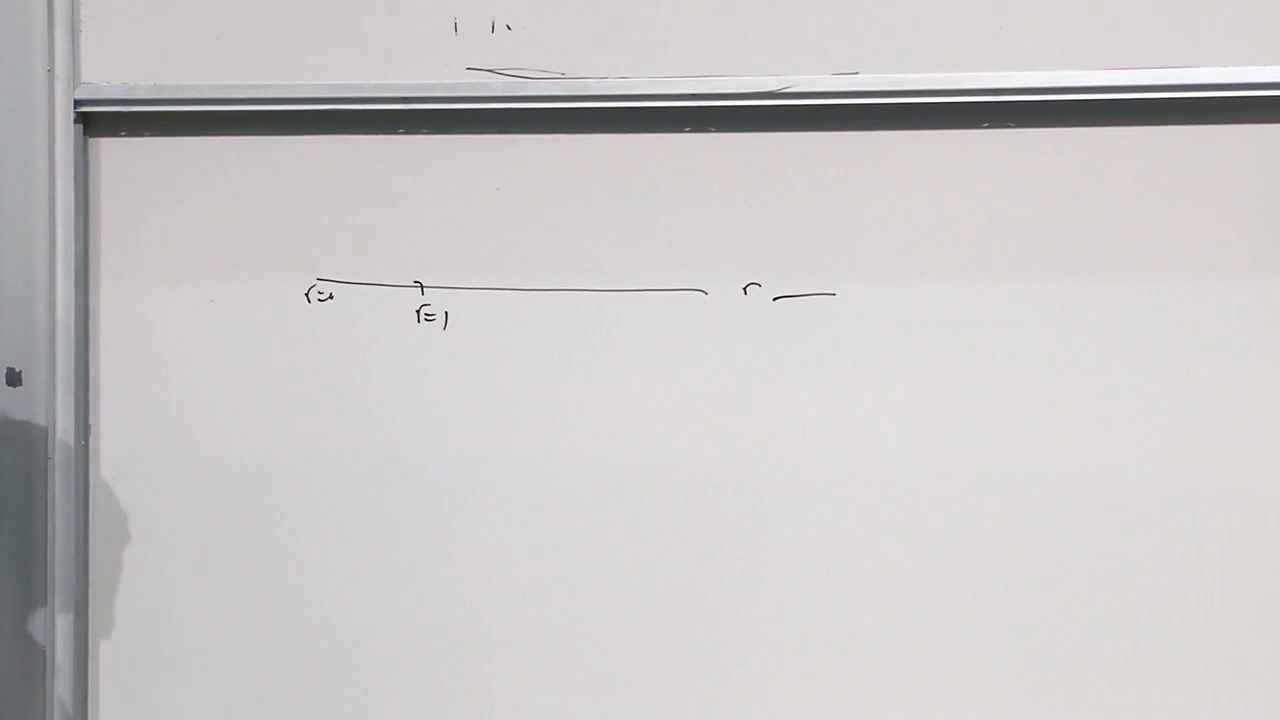
\includegraphics[width=0.78\textwidth]{lecture_07_figure_02.png}
\caption{La línea radial de coordenadas usada en la pizarra. El horizonte está en \(r=1\), mientras que \(r=0\) es la singularidad de curvatura.}
\lectureframe{00:16:11}
\end{figure}

Mantengamos fijos \(t\) y los ángulos. Entonces, el elemento de línea espacial positivo es
\begin{equation}
ds^2=\frac{dr^2}{1-\frac1r},
\qquad
ds=\sqrt{\frac{r}{r-1}}\,dr.
\label{eq:l7-radial-proper-line}
\end{equation}
Definamos la distancia propia adimensional al horizonte mediante
\begin{equation}
\rho(r)
=
\int_1^r\sqrt{\frac{r'}{r'-1}}\,dr'.
\label{eq:l7-rho-definition}
\end{equation}
Al restablecer la escala global, la distancia física es \(r_{\mathrm S}\rho\). No necesitaremos la forma cerrada de la integral. Solo necesitamos su derivada:
\begin{equation}
\frac{d\rho}{dr}
=\sqrt{\frac{r}{r-1}},
\qquad
d\rho^2
=\frac{dr^2}{1-\frac1r}.
\label{eq:l7-rho-derivative}
\end{equation}
Así, el complicado término radial se convierte exactamente en \(-d\rho^2\). Esa simplificación es la razón para introducir \(\rho\).

Ahora reescalemos una vez más la coordenada temporal,
\begin{equation}
\omega=\frac{t}{2}.
\label{eq:l7-omega}
\end{equation}
Como \(r\) es función de \(\rho\), podemos escribir la métrica como
\begin{equation}
d\tau^2
=
F(\rho)\rho^2d\omega^2
-
d\rho^2
-
r(\rho)^2d\Omega_2^2.
\label{eq:l7-rho-metric}
\end{equation}

\begin{classroomqa}
\audiencequestion{¿Se está definiendo simplemente \(F(\rho)\) de modo que el coeficiente temporal tenga la forma \(F(\rho)\rho^2\)?}
\lecturerresponse{Sí. En este punto, la factorización no tiene contenido físico independiente. Es una definición conveniente. Su utilidad se aprecia al tomar los límites de \(F\) cerca y lejos del horizonte.
\lecturetimestamp{00:26:39--00:26:59}}
\end{classroomqa}

Lejos, el coeficiente temporal de Schwarzschild tiende a uno. Como \(dt=2d\omega\), esto se convierte en
\begin{equation}
\lim_{\rho\to\infty}F(\rho)\rho^2=4.
\label{eq:l7-far-limit}
\end{equation}
Cerca del horizonte, la ec.~\eqref{eq:l7-rho-definition} da
\begin{equation}
\begin{aligned}
\rho&\simeq 2\sqrt{r-1},\\
r(\rho)&=1+\frac{\rho^2}{4}+O(\rho^4),\\
\lim_{\rho\to0}F(\rho)&=1.
\end{aligned}
\label{eq:l7-near-expansion}
\end{equation}

\begin{figure}[htbp]
\centering
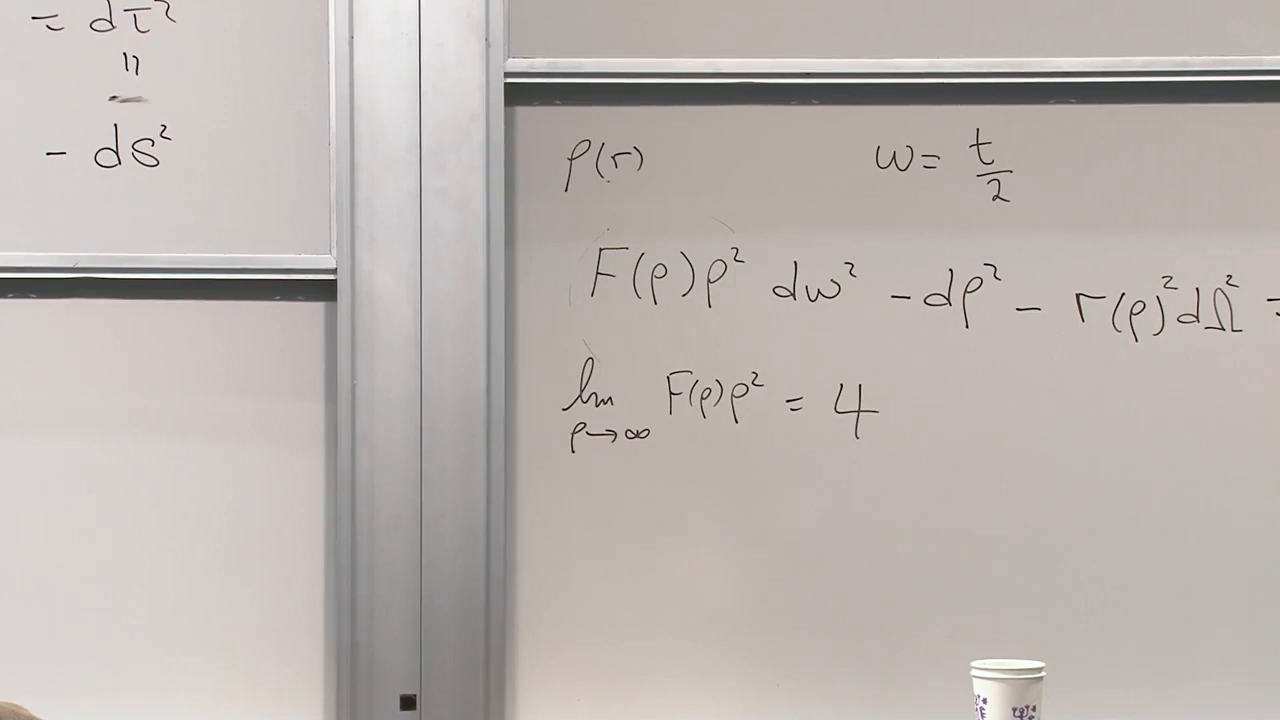
\includegraphics[width=0.90\textwidth]{lecture_07_figure_03.png}
\caption{La métrica en \((\rho,\omega)\), su coeficiente temporal asintótico y los límites cerca del horizonte \(F\to1\) y \(r=1+\rho^2/4+\cdots\).}
\lectureframe{00:37:30}
\end{figure}

\section{Espacio-tiempo plano oculto en el horizonte}

Cerca de \(\rho=0\), la parte radial-temporal de la ec.~\eqref{eq:l7-rho-metric} se reduce a
\begin{equation}
d\tau_{\mathrm{radial}}^2
\simeq
\rho^2d\omega^2-d\rho^2.
\label{eq:l7-rindler-metric}
\end{equation}
Este es el espacio-tiempo plano de Minkowski en coordenadas polares hiperbólicas. Definamos
\begin{equation}
X=\rho\cosh\omega,
\qquad
T=\rho\sinh\omega.
\label{eq:l7-rindler-transform}
\end{equation}
Entonces,
\begin{equation}
dT^2-dX^2
=
\rho^2d\omega^2-d\rho^2.
\label{eq:l7-minkowski-check}
\end{equation}
Las curvas de \(\rho\) constante satisfacen
\begin{equation}
X^2-T^2=\rho^2
\label{eq:l7-constant-rho}
\end{equation}
y son hipérbolas. Las curvas de \(\omega\) constante son rayos que parten del origen. Cuando \(\omega\to\infty\), esos rayos se aproximan a la recta nula \(T=X\). Por tanto, el horizonte de Schwarzschild, aparentemente relegado a un tiempo coordenado infinito, es una recta nula ordinaria en el diagrama regular.

\begin{figure}[htbp]
\centering
\includegraphics[width=0.88\textwidth]{lecture_07_figure_06.png}
\caption{La geometría completa de la pizarra: hipérbolas de \(\rho\) constante, rayos de \(\omega\) constante, el horizonte nulo y la región \(r<1\) por encima de él.}
\lectureframe{00:38:30}
\end{figure}

\begin{figure}[htbp]
\centering
\resizebox{0.96\linewidth}{!}{%
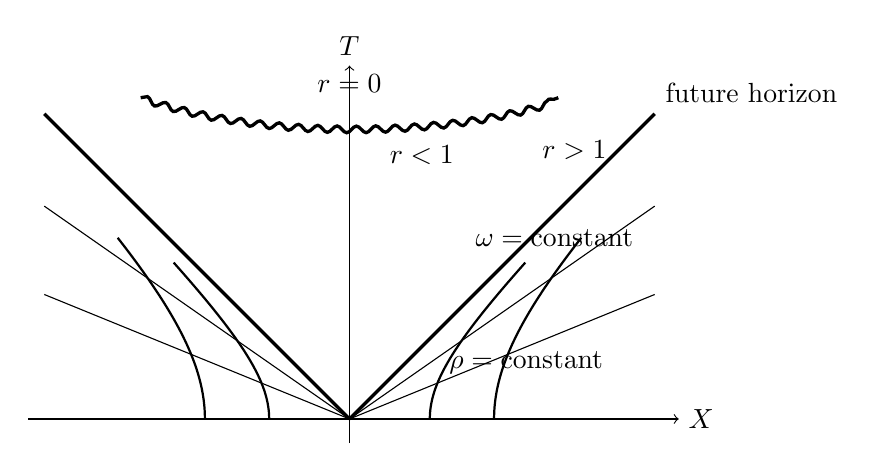
\begin{tikzpicture}[scale=1.02]
\draw[->] (-4.0,0) -- (4.1,0) node[right] {$X$};
\draw[->] (0,-0.3) -- (0,4.4) node[above] {$T$};
\draw[very thick] (0,0) -- (3.8,3.8)
  node[above right] {future horizon};
\draw[very thick] (0,0) -- (-3.8,3.8);
\draw[thick]
  plot[domain=0:1.42,samples=50]
  ({1.0*cosh(\x)},{1.0*sinh(\x)});
\draw[thick]
  plot[domain=0:1.05,samples=50]
  ({1.8*cosh(\x)},{1.8*sinh(\x)});
\draw[thick]
  plot[domain=0:1.42,samples=50]
  ({-1.0*cosh(\x)},{1.0*sinh(\x)});
\draw[thick]
  plot[domain=0:1.05,samples=50]
  ({-1.8*cosh(\x)},{1.8*sinh(\x)});
\draw[thin] (0,0) -- (3.8,1.55);
\draw[thin] (0,0) -- (3.8,2.65);
\draw[thin] (0,0) -- (-3.8,1.55);
\draw[thin] (0,0) -- (-3.8,2.65);
\draw[very thick,decorate,decoration={snake,amplitude=1.2pt,segment length=7pt}]
  (-2.6,4.0) .. controls (-1.2,3.5) and (1.2,3.5) .. (2.6,4.0);
\node at (0,4.18) {$r=0$};
\node at (2.2,0.7) {$\rho=\mathrm{constant}$};
\node at (2.55,2.25) {$\omega=\mathrm{constant}$};
\node at (0.9,3.28) {$r<1$};
\node at (2.8,3.35) {$r>1$};
\end{tikzpicture}
}
\caption{Una reconstrucción causal limpia. El horizonte es una recta nula, mientras que la singularidad de curvatura \(r=0\) es una frontera futura en el interior del agujero.}
\label{fig:l7-kruskal-clean}
\end{figure}

El límite de \(\rho\) pequeño difiere del límite de radio pequeño en coordenadas polares euclídeas. Un círculo euclídeo pequeño se contrae hasta un punto. Una hipérbola de \(\rho\) constante se aproxima a toda una recta nula. Así pues, \(\rho=0\) etiqueta el horizonte entero, no solo el punto donde se cruzan los ejes.

La expresión exterior puede continuarse analíticamente a \(r<1\). Cerca del horizonte, \(r-1\simeq\rho^2/4\), de modo que el interior corresponde formalmente a \(\rho^2<0\). Se puede llamar imaginario a \(\rho\), pero es más sencillo usar \(\rho^2\), \(r\) o las coordenadas regulares \(T,X\). Los signos de los coeficientes de Schwarzschild de \(t\) y \(r\) se intercambian en el interior. Eso no significa que el reloj de pulsera físico se convierta en una regla. Significa que las coordenadas de Schwarzschild han intercambiado su carácter causal.

\begin{classroomqa}
\audiencequestion{¿Qué son las hipérbolas horizontales dentro del horizonte y qué representan los rayos rectos?}
\lecturerresponse{Las curvas hiperbólicas son de \(r\) constante, o equivalentemente de \(\rho^2\) constante, prolongadas al interior de \(r<1\). Los rayos corresponden a tiempo de Schwarzschild constante. En el exterior forman una retícula de coordenadas útil; en el interior, no hay que confundir las mismas etiquetas con trayectorias de observadores físicos.
\lecturetimestamp{00:44:12--00:44:59}}
\end{classroomqa}

\begin{classroomqa}
\audiencequestion{¿La dirección vertical es una coordenada temporal y a qué marco de referencia corresponde?}
\lecturerresponse{Es una dirección temporal regular en el nuevo diagrama del espacio-tiempo, pero no es el tiempo de Schwarzschild singular \(t\). El diagrama está adaptado a la estructura causal de la caída libre. Un observador mantenido a radio exterior fijo sigue una hipérbola y debe acelerarse; un observador en caída libre atraviesa suavemente el horizonte nulo.
\lecturetimestamp{00:45:54--00:46:48}}
\end{classroomqa}

\begin{classroomqa}
\audiencequestion{Si \(\rho^2<0\) en el interior, ¿dónde aparece explícitamente el factor \(i\)?}
\lecturerresponse{Se puede introducir un \(\rho\) imaginario, pero no se gana nada con ello. El contenido invariante está en \(r\), en \(\rho^2\) y en las coordenadas reales regulares \(T,X\). La relación \(r-1\simeq\rho^2/4\) es solo la expansión cerca del horizonte.
\lecturetimestamp{00:52:35--00:53:00}}
\end{classroomqa}

En la clase, el diagrama regular suele describirse como la representación de Kruskal. En sentido estricto, las coordenadas exactas de Kruskal incluyen un factor radial que mantiene regular toda la métrica de Schwarzschild, mientras que la ec.~\eqref{eq:l7-rindler-transform} es su forma cerca del horizonte. El mensaje causal es el mismo: el horizonte es regular, pero toda curva temporal o nula dirigida hacia el futuro en el interior termina en \(r=0\). Ningún giro superlumínico puede hacerla volver a través del horizonte.

\subsection{Cómo se entendió la singularidad de coordenadas}

Históricamente fue difícil ver que el horizonte es regular porque las coordenadas originales de Schwarzschild hacen que sus coeficientes parezcan singulares. Eddington y, más tarde, Finkelstein introdujeron coordenadas que atraviesan el horizonte, y Finkelstein reconoció la frontera causal unidireccional. Kruskal, cuya habilidad para cambiar de coordenadas procedía de la física del plasma, proporcionó una representación global regular de la solución eterna.

La clase hace una pausa para hablar de John Wheeler, quien contribuyó a que la expresión «agujero negro» se volviera ineludible. La pausa es tanto personal como histórica: se recuerda a Wheeler como un amigo amable y reflexivo, aunque hubiera fuertes desacuerdos sobre juicios políticos, incluidos los relativos a la competencia nuclear. Se cuenta una anécdota personal humorística para evitar caricaturizar a Wheeler como alguien socialmente convencional. El punto técnico vuelve con la réplica: «los agujeros negros no tienen pelo». Un agujero sin rotación perturbado se asienta rápidamente hacia la simetría esférica; uno en rotación se asienta hacia la forma estacionaria determinada por sus parámetros conservados. Esta es la versión cualitativa de la idea de la ausencia de pelo que presenta la clase, no una demostración del teorema completo.

\section{Alice atraviesa el horizonte; Bob se queda fuera}

El diagrama extendido maximalmente contiene regiones que no aparecen en el espacio-tiempo sencillo de una estrella que colapsa a partir de datos iniciales ordinarios. Para el experimento con observadores solo usamos el exterior, el horizonte futuro y el interior del agujero negro.

\begin{figure}[htbp]
\centering
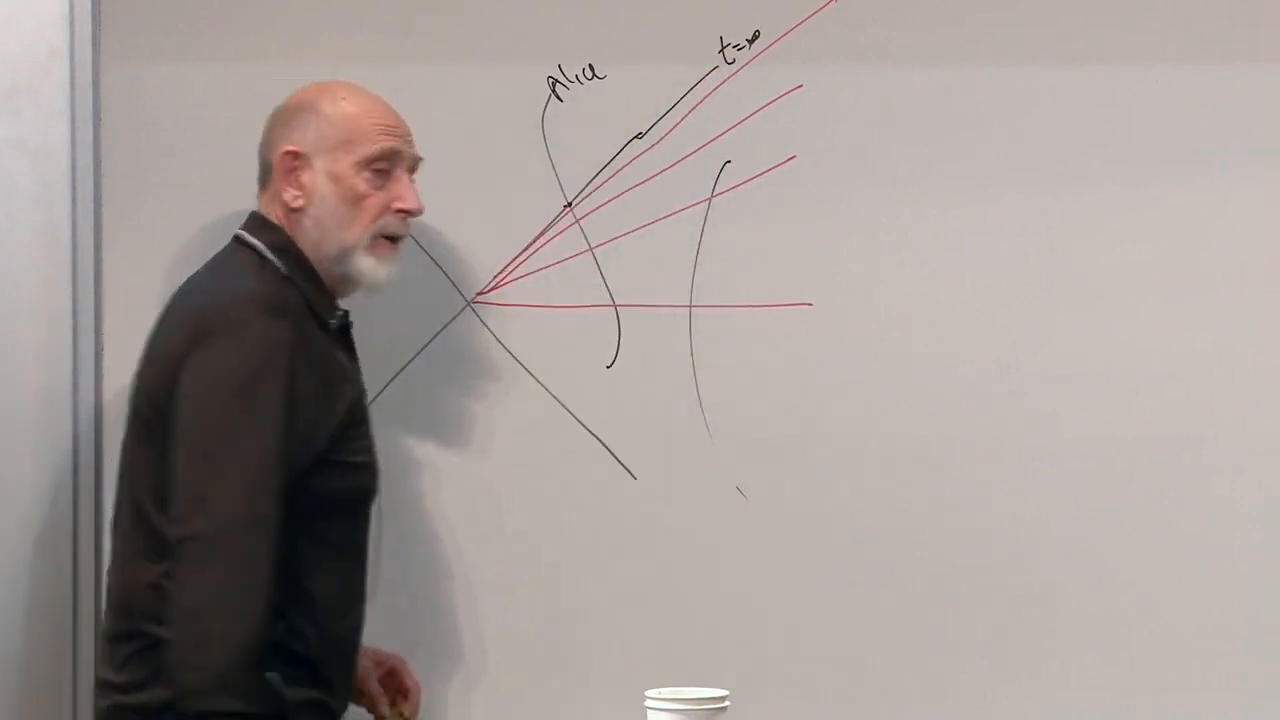
\includegraphics[width=0.84\textwidth]{lecture_07_figure_04.png}
\caption{La línea de universo de Alice en caída y los rayos de tiempo de Schwarzschild constante. El rayo límite está etiquetado \(t=\infty\).}
\lectureframe{00:54:54}
\end{figure}

Alice cae libremente. Su línea de universo atraviesa el horizonte y alcanza la singularidad en un tiempo propio finito. Su reloj no experimenta nada singular en el horizonte si el agujero negro es lo bastante grande como para que allí las fuerzas de marea sean pequeñas.

Bob, en cambio, permanece a un radio exterior fijo. Mantenerse allí requiere aceleración. La luz procedente de puntos cada vez más tardíos de la trayectoria de Alice le llega con retrasos crecientes y con un corrimiento al rojo cada vez mayor. En tiempo de Schwarzschild, Alice se aproxima a \(t=\infty\) y Bob nunca recibe una señal emitida después de que ella atraviese el horizonte. Son afirmaciones sobre señales causales y sobre la foliación exterior, no pruebas de que haya una superficie material en el horizonte.

\begin{classroomqa}
\audiencequestion{Si Bob ve que Alice se ralentiza, ¿Alice debe ver que Bob se acelera?}
\lecturerresponse{No. Alice sigue recibiendo señales luminosas ordinarias de Bob mientras dure su línea de universo. Hay un último suceso de la línea de universo de Bob que puede llegar hasta ella, pero es el último solo porque Alice alcanza después la singularidad. A Bob no le ocurre nada abrupto. La observación siempre mira dentro de un cono de luz pasado, y la relación causal entre las dos líneas de universo es asimétrica.
\lecturetimestamp{00:58:31--01:01:23}}
\end{classroomqa}

\begin{classroomqa}
\audiencequestion{Si Bob sabe que, en sus coordenadas, Alice sigue cerca del horizonte, ¿puede bajar, rescatarla y regresar?}
\lecturerresponse{Una línea de universo de rescate debe encontrarse con Alice antes de que ella atraviese el horizonte de sucesos. Después de ese suceso, ninguna trayectoria dirigida hacia el futuro puede encontrarse con ella y regresar al exterior. Que las foliaciones de Schwarzschild sitúen el cruce en \(t=\infty\) no significa que Alice permanezca sobre una superficie material de la que pueda ser rescatada; muestra que esas foliaciones no proporcionan una noción global de «ahora» a través del horizonte.
\lecturetimestamp{01:01:24--01:02:12}}
\end{classroomqa}

\section{Charlie sigue a Alice}

Hagamos que Charlie caiga a poca distancia detrás de Alice. Entonces, ambos son aproximadamente inerciales cerca del horizonte. Pueden intercambiar señales, conversar en ambas direcciones e incluso darse la mano. Ninguno ve una señal que marque el horizonte. La diferencia con Bob no es una diferencia entre tres personas con nombre. Es una diferencia entre la caída libre y una línea de universo acelerada que permanece en el exterior.

\begin{classroomqa}
\audiencequestion{¿Qué ve Bob si Alice cae primero y Charlie la sigue, como una pelota de baloncesto que sigue a un aro?}
\lecturerresponse{Bob ve que ambos se acercan al horizonte. Como va por delante, Alice parece ralentizarse progresivamente y comprimirse en la dirección radial antes que Charlie. Charlie parece acercarse cada vez más a ella, pero nunca la alcanza en la vista límite que Bob tiene desde el exterior. Esa acumulación visual no describe lo que siente ninguno de los dos observadores en caída.
\lecturetimestamp{01:04:12--01:06:05}}
\end{classroomqa}

\begin{classroomqa}
\audiencequestion{¿La aparente deformación aplanada contradice la fuerza de marea, que debería estirar radialmente al observador en caída?}
\lecturerresponse{Son efectos distintos. La deformación aplanada pertenece a la descripción de Bob en coordenadas de Schwarzschild. El alargamiento de marea es un efecto local de la curvatura que Alice y Charlie pueden sentir. La discusión de los observadores supone un agujero negro suficientemente grande, o unos observadores suficientemente pequeños, para que el efecto de marea en el horizonte sea despreciable. En cambio, un agujero de masa aproximadamente solar tendría mareas intensas en el horizonte, mientras que las de uno supermasivo pueden ser débiles.
\lecturetimestamp{01:06:07--01:08:18}}
\end{classroomqa}

\begin{classroomqa}
\audiencequestion{¿Ve Charlie a Alice atravesar el horizonte mientras él todavía está fuera?}
\lecturerresponse{Dibujemos el rayo nulo. La luz emitida cuando Alice cruza recorre el horizonte y llega a Charlie cuando él lo cruza. En ese suceso, puede calcular que ha visto el cruce de ella, aunque ninguno de los dos observadores encuentre una señal local. Después puede verla en el interior. Si acelera para alejarse antes de cruzar y logra permanecer fuera, nunca ve el cruce.
\lecturetimestamp{01:08:19--01:11:11}}
\end{classroomqa}

\begin{classroomqa}
\audiencequestion{Si Alice ya está dentro mientras Charlie está fuera, ¿cómo se pueden comparar sus radios posteriores y los tiempos de cruce?}
\lecturerresponse{No hay una relación de simultaneidad independiente del observador que pueda deducirse de una expresión como «al mismo tiempo». Alice ve a Charlie en su cono de luz pasado y solo puede ver su cruce posterior cuando ella se encuentra más adentro. Las líneas de universo y los rayos nulos concretos responden a la pregunta. Cualquier extrapolación general a muchos observadores en caída muy separados debe comprobarse dibujando su diagrama causal real, en lugar de suponer que existe un tiempo de cruce universal.
\lecturetimestamp{01:11:14--01:12:31}}
\end{classroomqa}

En las coordenadas regulares cercanas al horizonte, una trayectoria en caída libre es casi una recta. No es exactamente recta en la geometría completa de Schwarzschild, pero la aproximación es buena cerca de un horizonte grande y de curvatura débil.

\begin{classroomqa}
\audiencequestion{¿Puede la teoría de cuerdas determinar qué ocurre en el régimen de gravedad cuántica del interior de un agujero negro?}
\lecturerresponse{Es precisamente ahí donde el tema se vuelve sutil. Se necesita una teoría cuántica de la gravedad cerca de la singularidad, y la teoría de cuerdas es un marco candidato, pero las preguntas pertinentes seguían siendo difíciles y objeto de investigación activa; no se resolvían con una aplicación sencilla del diagrama clásico.
\lecturetimestamp{01:13:04--01:13:38}}
\end{classroomqa}

\begin{classroomqa}
\audiencequestion{¿Qué ocurre con el reloj y la velocidad de Alice cuando atraviesa el horizonte?}
\lecturerresponse{Su reloj sigue avanzando a su ritmo local ordinario y registra un tiempo propio finito. En su marco de reposo instantáneo está en reposo; con respecto a un marco local en caída libre tiene una velocidad finita ordinaria. Cerca de un horizonte grande, la geometría es casi plana, de modo que las marcas de tiempo propio a lo largo de su línea de universo siguen siendo regulares hasta que la curvatura se vuelve intensa cerca de la singularidad.
\lecturetimestamp{01:13:39--01:14:44}}
\end{classroomqa}

\begin{classroomqa}
\audiencequestion{¿Qué pasa si Bob acelera hacia el exterior, pero no lo suficiente como para evitar caer a través del horizonte?}
\lecturerresponse{Entonces su línea de universo se curva hacia el exterior, pero aun así atraviesa el horizonte. Si lo cruza muy tarde, puede ver a Alice poco después de su cruce, pero le queda poco tiempo propio antes de alcanzar la singularidad. Las pendientes de las líneas de universo en el dibujo no son escalas calibradas de distancia ni de tiempo; lo que se conserva es el orden causal, no sus longitudes euclídeas dibujadas.
\lecturetimestamp{01:14:47--01:16:31}}
\end{classroomqa}

Todas estas conclusiones suponen que ninguna señal supera la velocidad de la luz. La clase bromea brevemente sobre noticias de prensa de entonces, según las cuales unos neutrinos parecían superlumínicos en Italia; era una alusión a un error en la medición del tiempo experimental, no a una excepción a la relatividad. La construcción causal sigue estando limitada por las rectas nulas.

\begin{classroomqa}
\audiencequestion{¿Pueden unos relojes sincronizados que llevan Alice y Bob resolver la cuestión si Alice se lanza hacia el horizonte y regresa?}
\lecturerresponse{Pueden comparar sus relojes cuando coinciden, pero una vez que sus líneas de universo se separan no existe una sincronización distante única, sobre todo si uno de ellos cambia de movimiento. Dibujemos ambas líneas de universo y los rayos nulos intercambiados. Ese diagrama proporciona la respuesta operacional para cualquier experimento especificado.
\lecturetimestamp{01:17:34--01:18:25}}
\end{classroomqa}

\begin{figure}[htbp]
\centering
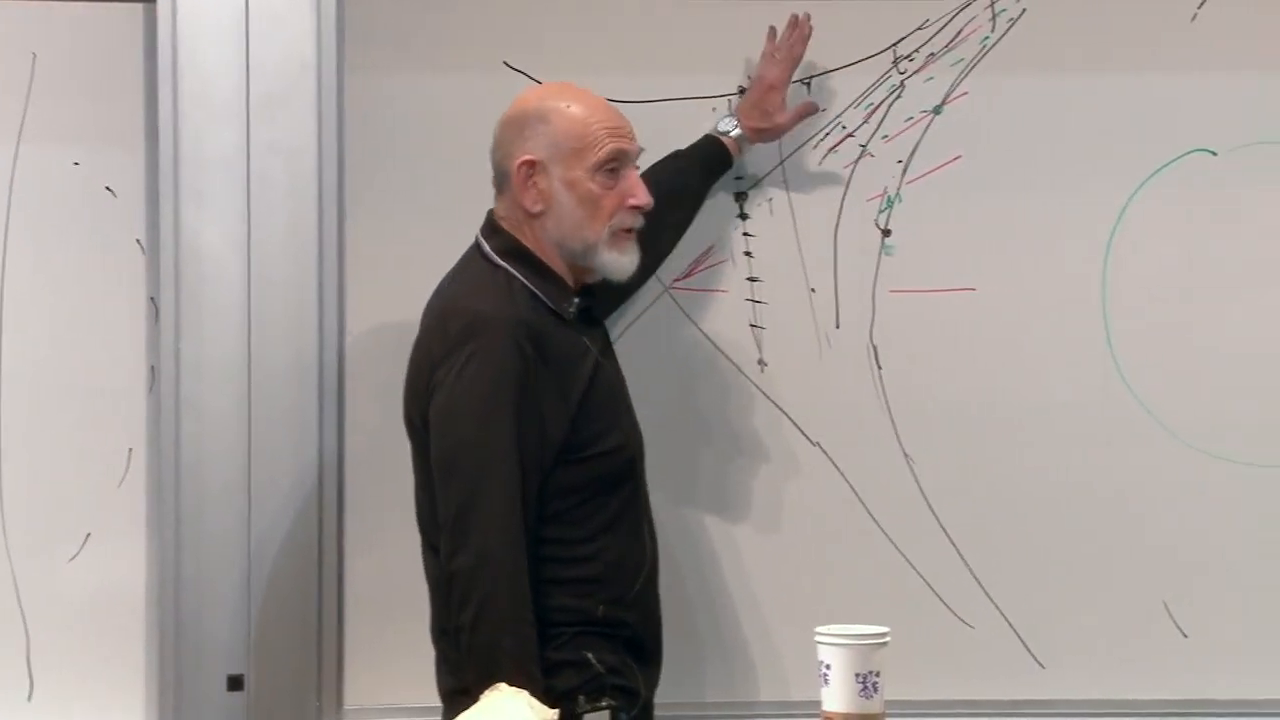
\includegraphics[width=0.86\textwidth]{lecture_07_figure_05.png}
\caption{El diagrama causal acumulado que se usa para responder a las preguntas sobre Alice, Bob y Charlie. Cada observación se localiza trazando un rayo nulo desde el suceso observado hasta la línea de universo del observador.}
\lectureframe{01:18:12}
\end{figure}

\begin{figure}[htbp]
\centering
\resizebox{0.96\linewidth}{!}{%
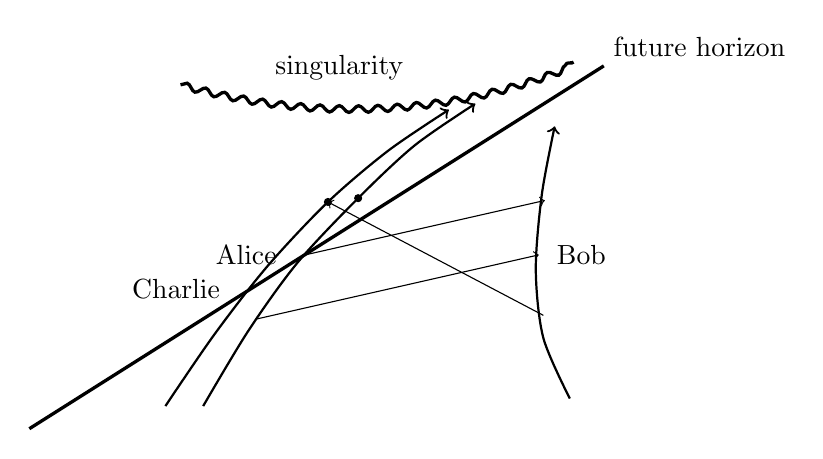
\begin{tikzpicture}[scale=0.96]
\draw[very thick] (-3.8,-0.3) -- (3.8,4.5);
\node[above right] at (3.8,4.5) {future horizon};
\draw[very thick,decorate,decoration={snake,amplitude=1.2pt,segment length=7pt}]
  (-1.8,4.25) .. controls (0.1,3.72) and (2.0,3.92) .. (3.4,4.55);
\node at (0.3,4.48) {singularity};
\draw[thick,->]
  plot[smooth] coordinates {(-1.5,0.0) (-0.9,1.0) (-0.25,1.9)
  (0.55,2.75) (1.3,3.45) (2.1,4.0)};
\node[left] at (-0.4,2.0) {Alice};
\draw[thick,->]
  plot[smooth] coordinates {(-2.0,0.0) (-1.35,0.95) (-0.65,1.85)
  (0.15,2.7) (0.95,3.38) (1.75,3.92)};
\node[left] at (-1.15,1.55) {Charlie};
\draw[thick,->]
  plot[smooth] coordinates {(3.35,0.1) (3.0,0.9) (2.9,1.8)
  (2.98,2.8) (3.15,3.7)};
\node[right] at (3.05,2.0) {Bob};
\draw[thin,->] (-0.8,1.15) -- (2.94,2.0);
\draw[thin,->] (-0.15,2.0) -- (3.02,2.72);
\draw[thin,->] (3.0,1.2) -- (0.15,2.7);
\draw[fill] (0.55,2.75) circle (1.3pt);
\draw[fill] (0.15,2.7) circle (1.3pt);
\end{tikzpicture}
}
\caption{Diagrama esquemático de los observadores. Las observaciones de Bob desde el exterior y las observaciones mutuas entre Alice y Charlie se construyen con rayos nulos diferentes; no son eslóganes recíprocos sobre relojes.}
\label{fig:l7-observers-clean}
\end{figure}

\begin{classroomqa}
\audiencequestion{¿Ve Bob a Alice durante un tiempo infinito, y significa eso que ella nunca muere en su realidad?}
\lecturerresponse{Bob recibe sus señales durante un intervalo ilimitado de su tiempo, pero ve cómo el ritmo del reloj de ella tiende a cero y solo recibe la secuencia finita de latidos emitidos antes de que ella cruce. La palabra «realidad» oculta la distinción entre un suceso local y el registro asintótico de un observador. Alice no experimenta que su reloj se detenga en el horizonte; el registro de Bob presenta retrasos y corrimientos al rojo cada vez mayores.
\lecturetimestamp{01:18:32--01:20:59}}
\end{classroomqa}

\begin{classroomqa}
\audiencequestion{¿Ve Alice de repente toda la materia antigua que parecía congelada en el horizonte cuando lo atraviesa?}
\lecturerresponse{No se produce ninguna aclaración repentina. A medida que cae, los conos de luz pasados desde los que ve la materia anterior cambian continuamente. Puede deducir que la luz que le llega ahora se emitió antes y que la materia atravesó el horizonte antes que ella. La perspectiva de Charlie sobre Alice enseña lo mismo: ninguno de los cruces produce una discontinuidad local ni revela un montón oculto de sillas y dinosaurios.
\lecturetimestamp{01:21:02--01:23:48}}
\end{classroomqa}

\begin{classroomqa}
\audiencequestion{¿Hay simulaciones realistas de lo que vería un observador en caída?}
\lecturerresponse{La clase remite a las visualizaciones de agujeros negros de Andrew Hamilton. Pueden transmitir la intensa aberración y los desplazamientos de frecuencia de la luz entrante, aunque la imagen quizá desoriente más de lo que aclara. «En el horizonte no ocurre nada especial» se refiere a la geometría local, no a que el cielo tenga un aspecto corriente.
\lecturetimestamp{01:24:11--01:25:29}}
\end{classroomqa}

\section{De un agujero eterno a uno que crece}

El vértice inferior del diagrama eterno extendido maximalmente tiene poca relevancia directa para un agujero negro formado por el colapso de una estrella. En la geometría sencilla del colapso solo aparece la parte que contiene el exterior, el horizonte futuro y el interior futuro. Esta distinción se vuelve esencial cuando se permite que la materia cambie la masa del agujero.

\begin{classroomqa}
\audiencequestion{¿Qué suceso físico representa el vértice inferior del diagrama idealizado?}
\lecturerresponse{En la solución matemática eterna, forma parte de la extensión maximal. Un agujero negro formado por materia en colapso no contiene toda esa región inferior. Su horizonte tiene una historia de formación, que requiere un diagrama global distinto y se desarrolla en la siguiente clase.
\lecturetimestamp{01:25:59--01:26:52}}
\end{classroomqa}

Cuando cae un cuerpo de prueba pequeño, se puede despreciar su reacción y basta con el diagrama de Schwarzschild fijo. Si cae una masa considerable, aumentan la masa del agujero negro y el radio de Schwarzschild:
\begin{equation}
r_{\mathrm S}=2GM,
\qquad
\Delta r_{\mathrm S}=2G\,\Delta M.
\label{eq:l7-growing-radius}
\end{equation}
El horizonte se deforma hacia el objeto entrante, los horizontes se unen y el horizonte común deformado se estabiliza rápidamente. En la idealización sin rotación de la clase, el estado final es una esfera un poco mayor. Una fusión real también irradia energía en forma de ondas gravitacionales y, en general, deja un agujero negro en rotación.

\begin{classroomqa}
\audiencequestion{Si el horizonte crece cuando cae masa, ¿se desplaza hacia afuera para alcanzar la materia que parecía congelada cerca del horizonte anterior?}
\lecturerresponse{Para un objeto en caída suficientemente masivo, deja de ser válida la descripción de partícula de prueba. El horizonte se deforma, se une a la región atrapada del objeto entrante y se relaja hasta convertirse en un horizonte estacionario mayor. La ubicación exacta del horizonte de sucesos es global y puede extenderse a una región anterior a la llegada de la materia en caída. La clase aplaza deliberadamente la construcción completa hasta la próxima sesión.
\lecturetimestamp{01:26:55--01:29:05}}
\end{classroomqa}

\begin{classroomqa}
\audiencequestion{¿Por qué pueden ver destellos los astrónomos si se dice que la materia tarda un tiempo de Schwarzschild infinito en llegar al horizonte?}
\lecturerresponse{La radiación brillante no procede del horizonte mismo. El gas de un flujo o disco de acreción choca y se calienta fuera del horizonte, incluso cerca de órbitas fotónicas intensas. Ese plasma exterior puede emitir luz que nos llega. La geometría vacía de Schwarzschild aísla el problema causal, pero no constituye un modelo completo de un entorno astrofísico.
\lecturetimestamp{01:29:07--01:30:22}}
\end{classroomqa}

La escala temporal característica de relajación viene determinada por el tiempo que tarda la luz en atravesar el agujero:
\begin{equation}
t_{\mathrm{cross}}\sim\frac{r_{\mathrm S}}{c},
\qquad
t_{\mathrm{relax}}\sim
\text{a few to a few tens of }t_{\mathrm{cross}}.
\label{eq:l7-relaxation-scale}
\end{equation}
La clase estima que \(10^{-5}\,\mathrm{s}\) es el tiempo de cruce de un agujero de escala kilométrica, y que se necesitan aproximadamente \(10^{-3}\,\mathrm{s}\) para que una fusión pequeña se vuelva casi estacionaria. Para un agujero de mil millones de masas solares, el tiempo correspondiente se mide en minutos u horas. Son estimaciones de escala, no cálculos precisos de fusiones. Lo importante es la secuencia geométrica: mancuerna, cacahuete, casi esférico, estacionario.

\begin{classroomqa}
\audiencequestion{¿Con qué rapidez se estabiliza un horizonte deformado o recién fusionado?}
\lecturerresponse{En una escala temporal que no es mucho mayor que el tiempo que tarda la luz en atravesar el agujero. Como todas las longitudes y tiempos escalan con \(r_{\mathrm S}\), los agujeros pequeños se estabilizan en fracciones de segundo y los supermasivos en tiempos de reloj mucho más largos. La afirmación de que no hay pelo describe el estado estacionario final; la deformación transitoria libera energía mediante radiación gravitacional.
\lecturetimestamp{01:30:26--01:33:18}}
\end{classroomqa}

\begin{classroomqa}
\audiencequestion{¿Qué ve Bob si hay materia anterior entre el horizonte antiguo y el nuevo mientras cae otro cuerpo pesado?}
\lecturerresponse{Esa pregunta no puede responderse de manera coherente ensamblando dos diagramas estáticos de Schwarzschild. Hay que resolver o construir la geometría del colapso dependiente del tiempo y localizar su horizonte global. La clase deja abierta la pregunta y aplaza explícitamente la respuesta hasta la semana siguiente, cuando se tratará la formación del horizonte.
\lecturetimestamp{01:33:20--01:35:41}}
\end{classroomqa}

\section{¿Qué cambia al cambiar la escala?}

El diagrama adimensional no cambia cuando cambia \(r_{\mathrm S}\). Lo que cambia es el significado físico de un intervalo dibujado:
\begin{equation}
d\tau_{\mathrm{physical}}^2
=
r_{\mathrm S}^2\,d\hat{\tau}^2,
\qquad
\ell_{\mathrm{physical}}
=
r_{\mathrm S}\,\hat{\ell}.
\label{eq:l7-scale-restoration}
\end{equation}
Una separación adimensional que representa medio kilómetro para un agujero de escala kilométrica representa aproximadamente medio millardo de kilómetros para un agujero mil veces mayor. Vuelve la analogía de las esferas dibujadas a la misma escala: la forma no cambia, mientras que el número de metros que representa una línea crece en proporción al radio.

\begin{classroomqa}
\audiencequestion{¿Cómo cambia el diagrama causal al cambiar el radio de Schwarzschild?}
\lecturerresponse{No cambia una vez que se ha eliminado la escala del radio. Todas las longitudes y tiempos físicos asignados al diagrama se multiplican por \(r_{\mathrm S}\), mientras que la curvatura en puntos adimensionales correspondientes se multiplica por \(r_{\mathrm S}^{-2}\).
\lecturetimestamp{01:35:41--01:38:10}}
\end{classroomqa}

\begin{classroomqa}
\audiencequestion{¿Cambia la conclusión causal si Bob está en órbita en vez de permanecer en reposo en una posición angular fija?}
\lecturerresponse{Los corrimientos al rojo detallados y las direcciones de llegada se vuelven más complicados, pero la separación causal del horizonte no cambia. Ninguna órbita temporal en el exterior recibe una señal emitida desde el interior del horizonte.
\lecturetimestamp{01:38:12--01:38:26}}
\end{classroomqa}

\begin{classroomqa}
\audiencequestion{Como la gravedad se anula dentro de una capa esférica, ¿se anula dentro del horizonte porque la masa del agujero negro está distribuida sobre esa superficie?}
\lecturerresponse{No. El horizonte de sucesos no es una capa material que contenga la masa. Por tanto, el teorema newtoniano de la capa esférica no se aplica a él. En la clase se compara la solución estática exterior con una fuente puntual situada en la singularidad de curvatura, pero la materia que está cayendo durante la formación requiere la geometría dependiente del tiempo que se tratará en la próxima clase.
\lecturetimestamp{01:38:28--01:40:41}}
\end{classroomqa}

\section{Rotación y geometría radial}

El momento angular sobrevive al colapso. La geometría exterior de un agujero negro en rotación difiere de la de Schwarzschild: su solución estacionaria es la de Kerr, la rotación deforma la geometría del horizonte y el arrastre de los marcos de referencia hace girar las direcciones inerciales alrededor del agujero. En principio, el momento angular se mide a partir de esos efectos gravitatorios exteriores. La materia con momento angular no lo pierde por el mero hecho de cruzar un horizonte.

\begin{classroomqa}
\audiencequestion{¿Puede un agujero negro tener un momento angular medible, y la rotación modifica la gravedad en su exterior?}
\lecturerresponse{Sí. El momento angular permanece como parámetro conservado, deforma la geometría estacionaria y produce arrastre de los marcos de referencia. El horizonte ya no es el sencillo horizonte esférico de Schwarzschild. En la clase se compara cualitativamente la deformación con la forma achatada de la Tierra, aunque se señala que la solución completa en rotación es mucho más complicada.
\lecturetimestamp{01:40:45--01:42:36}}
\end{classroomqa}

\begin{classroomqa}
\audiencequestion{¿Significa la relación entre \(r\) y la distancia propia
\(\rho\) que la gravedad contrae el espacio?}
\lecturerresponse{La distancia radial propia \(\rho\) satisface
\begin{equation*}
\frac{d\rho}{dr}=\sqrt{\frac{r}{r-1}}>1
\end{equation*}fuera del horizonte unitario. Por tanto, un incremento coordenado dado \(dr\) corresponde a un intervalo radial propio mayor cerca del horizonte. Decir que el espacio se contrae o se estira depende de qué intervalos coordenados se comparen. La afirmación invariante es la propia relación entre distancia propia y coordenada.
\lecturetimestamp{01:42:36--01:43:20}}
\end{classroomqa}

\section{Preguntas finales}

\begin{classroomqa}
\audiencequestion{Desde el punto de vista de Bob, el reloj de Alice parece detenerse. Desde el punto de vista de Alice, ¿llegan a su fin el espacio o el tiempo de Bob?}
\lecturerresponse{No. Alice ve señales ordinarias procedentes de sucesos sucesivos en la línea de universo de Bob hasta que termina su propia línea de universo. No ve sucesos posteriores de Bob porque no existe ningún punto posterior en su línea de universo, no porque Bob o su espacio desaparezcan. En estas coordenadas causales regulares, los rayos nulos radiales se representan como líneas rectas; que aparezcan como trayectorias curvas en otro sistema de coordenadas no altera qué sucesos conectan.
\lecturetimestamp{01:43:21--01:45:20}}
\end{classroomqa}

La relatividad general plantea dos tareas complementarias. Dada una métrica, se pueden trazar geodésicas y rayos nulos para determinar qué miden los observadores. Dada una distribución de materia, hay que resolver las ecuaciones de Einstein para hallar la métrica. Esta clase se ha centrado en la primera tarea. La segunda suele ser más difícil, aunque el colapso simétrico ofrece ejemplos tratables.

\begin{classroomqa}
\audiencequestion{¿Qué ocurre con el horizonte y la singularidad de un agujero negro que se evapora?}
\lecturerresponse{La clase presenta un esquema en el que el horizonte se contrae y se encuentra con el extremo de la región singular. La evaporación es un proceso cuántico semiclásico, y el estado final a escala de Planck no queda determinado por el diagrama clásico de Schwarzschild. Por tanto, el esquema de contracción debe entenderse como un anticipo cualitativo, no como una geometría cuántica completa.
\lecturetimestamp{01:46:04--01:46:32}}
\end{classroomqa}

Casi todos los agujeros negros astrofísicos deberían estar en rotación. Las estrellas ya poseen momento angular, y el colapso amplifica su velocidad angular, como cuando una patinadora acerca los brazos al cuerpo. La estructura singular de un agujero negro de Kerr no es la superficie \(r=0\) de Schwarzschild dibujada aquí, y no debe describirse como materia que literalmente gira a velocidad lineal infinita.

\begin{classroomqa}
\audiencequestion{¿Son comunes los agujeros negros macroscópicos sin rotación, y cuántos agujeros negros hay?}
\lecturerresponse{Un momento angular exactamente nulo sería una idealización excepcional. En la clase se ofrece solo una estimación didáctica de orden de magnitud para la población cósmica, situada entre el número de galaxias y el de estrellas y quizá en torno a \(10^{15}\). Es una estimación de la época de la clase, no un censo medido. La idea sólida es que, en general, el colapso conserva y amplifica cierto momento angular.
\lecturetimestamp{01:46:32--01:48:42}}
\end{classroomqa}

\begin{classroomqa}
\audiencequestion{¿Se forman los agujeros negros a partir de materia existente o aparecen mediante un proceso cuántico?}
\lecturerresponse{Los agujeros negros astrofísicos ordinarios se forman cuando colapsa materia estelar existente. La fusión nuclear y el flujo de energía hacia el exterior ayudan a sostener una estrella. Cuando se agota el combustible, el remanente se contrae. Según su masa y el soporte de presión disponible, puede convertirse en una enana blanca, una estrella de neutrones o, si ningún soporte puede detener el colapso, cruzar su propio radio de Schwarzschild y formar un agujero negro.
\lecturetimestamp{01:48:43--01:50:23}}
\end{classroomqa}

\begin{classroomqa}
\audiencequestion{¿Podrían formarse agujeros negros microscópicos, y qué determinaría su vida y su tamaño mínimo?}
\lecturerresponse{Esta parte es especulativa. La evaporación de Hawking es más rápida cuanto menor es la masa, y la vida del agujero escala aproximadamente como \(M^3\). En la clase se compara con una montaña la masa de un agujero cuya vida podría ser cosmológica; la analogía numérica es solo aproximada. Las fluctuaciones violentas de densidad en el universo temprano o las colisiones suficientemente energéticas son posibles mecanismos de formación. Un agujero negro de masa cercana a la de Planck, aproximadamente \(10^{-5}\,\mathrm{g}\), marca la escala en la que una descripción geométrica clásica deja de ser fiable. Alcanzar esa energía con un acelerador convencional requeriría una máquina inverosímilmente grande si se extrapola de manera directa, aunque la formación es posible en principio.
\lecturetimestamp{01:50:23--01:53:31}}
\end{classroomqa}

\begin{classroomqa}
\audiencequestion{¿Se tratarán en el curso la cosmología, la materia oscura, la energía oscura, la entropía y las ondas gravitacionales?}
\lecturerresponse{Las aplicaciones cosmológicas y quizá las ondas gravitacionales podrían ser temas posteriores. La entropía de los agujeros negros se deja para después del trimestre. La clase termina reconociendo que esa tarde solo se cubrió aproximadamente una cuarta parte del material previsto: resolver las preguntas con cuidado importa más que recorrer a toda prisa el temario.
\lecturetimestamp{01:53:33--01:54:38}}
\end{classroomqa}

La regla operativa resiste todas las preguntas planteadas en el aula. Especifica las líneas de universo, traza los rayos nulos y localiza los eventos que conectan. El horizonte no es un lugar donde deje de funcionar la física local; es la frontera más allá de la cual toda señal dirigida al futuro permanece en el interior. La próxima clase sustituye el fondo eterno por una fuente en colapso y muestra cómo se forma esa frontera.